\chapter{State of the Art of SSI} \label{ch:ssi}

As mentioned in earlier chapters, the principle of \gls{ssi} has become popular in contemporary times, particularly in the context of cybersecurity and 
identity management. \gls{ssi} follows the decentralized method of managing digital identities, resulting in increased personal control and independence for individuals. 

In this chapter, we discuss current status of the \gls{ssi} model in the state-of-the-art. First, we give a historical background and then follow with an examination of evolution 
of \gls{ssi}. Next we focus on its architecture with an in-depth look at its core components and operational steps. Through this sector, we look to furnish a full picture of the 
identity management framework and the \gls{ssi} model in particular.

\section{History of Self-Sovereign Identity}

\subsection{Origins of SSI}

The roots of \gls{ssi} can be traced back to the early 90s with the introduction of encryption methods like \gls{pgp} by Phil 
Zimmerman \cite{businessreporter}. \gls{pgp} introduced the public key type of encryption, which formed the basis of later models of \gls{ssi}. \gls{pgp} allowed the users to directly 
exchange cryptographic keys, and, thus, enabled the creation of a network of trust without any need for centralized intermediaries.

\subsection{The Seven Laws of Identity}

The "Seven Laws of Identity" of Kim Cameron was pivotal in the development of \gls{ssi} approach in 2005 \cite{8776589}. These laws described the main building blocks of the user-oriented 
and conducive identity framework. The Seven Laws of Identity articulate key principles guiding \gls{ssi}, including:

\begin{enumerate}
  \item \textbf{User control and consent}: Technical identity systems must only reveal information identifying a user with the user’s consent.
  \item \textbf{Minimum disclosure for a constrained use}: The solution which discloses the least amount of identifying information and best limits its use is the most 
  stable long-term solution.
  \item \textbf{Justifiable Parties}: Digital identity systems must be designed so the disclosure of identifying information is limited to parties having a necessary and 
  justifiable place in a given identity relationship.
  \item \textbf{Directed Identity}: A universal identity system must support both “omni-directional” identifiers for use by public entities and “unidirectional” identifiers 
  for use by private entities, thus facilitating discovery while preventing unnecessary release of correlation handles.
  \item \textbf{Pluralism of Operators and Technologies}: A universal identity system must channel and enable the inter-working of multiple identity technologies run by 
  multiple identity providers.
  \item \textbf{Human Integration}: The universal identity metasystem must define the human user to be a component of the distributed system integrated through unambiguous 
  human-machine communication mechanisms offering protection against identity attacks.
  \item \textbf{Consistent Experience Across Contexts}: The unifying identity metasystem must guarantee its users a simple, consistent experience while enabling separation 
  of contexts through multiple operators and technologies.
\end{enumerate}

\subsection{Modern Development}

Christopher Allen had also made the term \gls{ssi} more popular than ever with his 2016 article "The Road to Self-Sovereign Identity" \cite{businessreporter}. Allen’s work 
was built on Cameron’s principles that highlighted the crucial aspects of user control, longevity, portability and limited disclosure in \gls{ssi} frameworks. These principles 
constitute the foundation of a system that is about individuals having the ultimate power over their personal information.

For the last few years, an increase in the use of blockchain technology has led to a rapid development of \gls{ssi}. With blockchain being a decentralized and
immutable system, it forms the backbone of \gls{ssi} systems that secures digital identities due to their immutable and transparent nature. \gls{did} and \gls{vc} are 
among others some of the components of modern \gls{ssi} architectures, which enables peer-to-peer transactions and having no need of central authorities.

\section{Advantages and Principles}

\subsection{Advantages of Decentralized Identity }

\subsubsection{Advantages for Organizations}

\begin{itemize}
    \item \textbf{Efficient Verification}: Organizations thus can verify information faster without involving the manual verification procedures, improving operational efficiency \cite{dockio}.
    \item \textbf{Prevention of Certificate Fraud}: Decentralized identity systems prevent abuse of fake certificates minimizing the chances of credentials being forged .
    \item \textbf{Enhanced Data Security}: Public-key cryptography is utilized by organizations to encrypt data safely, which therefore helps reduce the risk of data breaches.
    \item \textbf{Reduced Cybersecurity Risks}: Minimizing user data information makes organizations less sensitive to cybersecurity attacks. The overall cybersecurity posture improves.
\end{itemize}

\subsubsection{Advantages for Individuals}

\begin{itemize}
    \item \textbf{Data Ownership and Control}: People retain both ownership and control of their data, and they can independently manage their digital identities \cite{dockio}.
    \item \textbf{Self-Verification}: Individuals can establish their statements without the help of third parties, thus confidence and autonomy are promoted.
    \item \textbf{Privacy Protection}: Decentralized identity management provides better privacy because it can shield from indiscriminate tracking and allows for selective 
    disclosing of data.
    \item \textbf{Immutable Identity}: Identities will be stored and kept in the decentralized digital wallets in which they cannot be arbitrarily deleted and provide every 
    person with a reliable digital persona.
\end{itemize}

\subsubsection{Advantages for Developers}

\begin{itemize}
    \item \textbf{Enhanced User Experience}: The developers can build applications for users with short and easy user identification processes, resulting in increased ease of use.
    \item \textbf{Privacy-Preserving Data Requests}: Developers can request the data directly from users while respecting their privacy and increasing trust-users and transparency.
    \item \textbf{Streamlined Transactions}: Developers can simplify transactions by reaching the relevant information securely via decentralized identity wallets 
    without any time-consuming data collection activities \cite{dockio}.
\end{itemize}

\subsection{Principles of SSI }

\subsubsection{Foundational Properties}

\begin{itemize}
    \item \textbf{Existence}: People can digital assets for their characteristics which exist in the digital domain. This is what the \gls{ssi} achieves \cite{9869618}.
    \item \textbf{Autonomy}: \gls{ssi} provides full independence for self-governance in identity management to issue, edit, and revoke digital identities independently.
    \item \textbf{Ownership}: Users as the final decision-makers own their identities, including self-asserted and third-party-attributed claims.
    \item \textbf{Access}: Users don't have to worry about their identity; they can freely control when it is needed.
    \item \textbf{Single Source}: Since individuals are the single point of reference for their identities, they also prevent unauthorized information exchange without their consent.
\end{itemize}

\subsubsection{Security Properties}

\begin{itemize}
    \item \textbf{Protection}: \gls{ssi} provides strong protection via cryptographic means, thus ensuring trustworthiness, privacy and integrity of stored information.
    \item \textbf{Availability}: Readily accessible identities must be cross-platform compatible, while being resistant and recoverable \cite{9869618}.
    \item \textbf{Persistence}: Identities should be preserved as long as needed, protected through secure identity storage and transmission.
\end{itemize}

\subsubsection{Controllability Properties}

\begin{itemize}
    \item \textbf{Choosability}: Potential users could decide what data relating to identity they ought to disclose, granting access to information only in line with their preferences.
    \item \textbf{Disclosure}: Users have the luxury of sharing identifiable data in a selective manner to third party as long as it is done in a structured way that allows
    for fine-grained control \cite{9869618}.
    \item \textbf{Consent}: Identity information is delegated only with user consent, ensuring privacy protection and personal autonomy.
\end{itemize}

\subsubsection{Flexibility Properties}

\begin{itemize}
    \item \textbf{Portability}: The identity projects need the portability across platforms in order to ensure its longevity and inter-operability.
    \item \textbf{Interoperability}: Maximum interoperability should be achieved by \gls{ssi} systems, which in that case would allow for effortless communication with 
    existing identity systems \cite{9869618}. 
    \item \textbf{Minimization}: User objectives are meant to be covered, which minimizes data disclosure, thus ensuring data protection and efficiency of the data processing.
\end{itemize}

\subsubsection{Sustainability Properties}

\begin{itemize}
    \item \textbf{Transparency}: \gls{ssi} should be transparent, open-source, and accessible, which will produce trust, and participation of the community
    \item \textbf{Standardization}: The Identity should be compliant with open standards that enables it to have better portability and interoperability.
    \item \textbf{Cost}: Identity solutions should be cost-effective or free to make them affordable and that can lead to their wide adoption and inclusivity \cite{9869618}.
\end{itemize}

\section{Key Components of SSI} \label{sec:4.3}

This section elaborates on the three main pillars of \gls{ssi} model, each of which is of critical relevance to the revolution of digital identity management. We shall properly 
discuss \gls{did}s, \gls{vc}s, and Verifiable Data Registries, highlighting their importance and functionality in the identity 
ecosystem which is decentralized.

\subsection{Decentralized Identifiers}

\gls{did}s represents a cutting edge feature of \gls{ssi}. Unlike the conventional identifiers such as emails and usernames that are 
centralized, \gls{did}s provides a secure and decentralized way of verifying digital identities. \gls{did}sis an individual identifier, which can be used separately for people, 
organizations, and data models, without the need of any centralized authority. \gls{did}s are owned by users and are held in identity wallets, enabling people to retain control 
of their original data verified by certified issuers. \cite{ciscofpie} They are as well a solution to some of the problems linked to centralized identifiers such as identity theft and data 
leakage. Significantly, \gls{did}s do not contain personally identifiable information, that is why they are secure \cite{9333997}. 

\subsubsection{Syntactic Components of DIDs}

\gls{did}s are composed of distinct syntactic components, delineating their structure and facilitating interoperability across decentralized systems \cite{w3didcore} :

\begin{itemize}
  \item \textbf{Schema}: The schema serves as a guideline to provide a uniform structure and format of the \gls{did}s thereby ensuring compatibility to standardized conventions 
  and guidelines. These frameworks are mostly created by organizations like the \gls{w3c}, and they provide a bedrock for the deployment of \gls{did}s across
  various ecosystems.
  \item \textbf{Method}: Method part defines a protocol or mechanism used for creating and maintaining \gls{did}s within a certain ecosystem. Varying methods may involve different
  cryptographic algorithms or diverse distributed ledger technologies to develop and complete \gls{did}s. Examples of methods are "ethr" for EthDIDs-based \gls{did}s and "key" for 
  standard key-based \gls{did}s.
  \item \textbf{DID Method-Specific Identifier}: This identifier being unique for this method, differentiates the corresponding \gls{did}s within the indicated ecosystem. It 
  works as the reference point on \gls{did} documents finding and network interactions enabling within the decentralized systems.
\end{itemize}

\begin{figure}[h]  
  \centering
  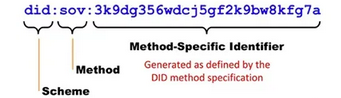
\includegraphics[width=0.6\textwidth]{Images/c4_1.png} 
  \caption{Decentralized Identifiers (DID) URI syntax.}
\end{figure}

\subsubsection{DID Document}

A \gls{ddo} outlines the basic details connected to a certain \gls{did}, being the main part of the identity system. It typically includes \cite{9869618}:

\begin{itemize}
  \item \textbf{Verification Methods}: Public keys or cryptographic objects serving as authentication and verification purposes.
  \item \textbf{Authentication Methods}: Holder of the \gls{did} is verified through specific validation mechanisms applied.
  \item \textbf{Service Endpoints}: Identifiers referring to services or endpoints associated with \gls{did} subject, allowing interactions and data exchange to be completed.
  \item \textbf{Timestamps}: Proof data records, which host the verification history data or temporal metadata, enhancing transparency and auditability.
  \item \textbf{Signature}: Cryptographic signatures used for the purpose of security and trust of the \gls{ddo}.
\end{itemize}

\subsubsection{DID Resolution}

\gls{did} resolution is the procedure for transforming a \gls{did} into the corresponding \gls{ddo} that allows for retrieval of information related to a particular \gls{did}. This 
procedure of querying distributed ledgers or repositories seeks the relevant \gls{ddo} \cite{w3didcore}. Upon the resolution, verifiers obtain crucial attributes and secure materials, 
thus being able to have secure interactions and identity verification within the delegated systems. In addition to that, \gls{did} resolution enables interoperability by 
standardizing mechanisms for use of \gls{did} associated data as well as for its access and interpretation.

\begin{figure}[h]  
  \centering
  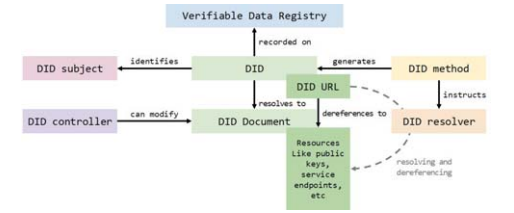
\includegraphics[width=0.8\textwidth]{Images/c4_2.png} 
  \caption{The basic components of DIDs architecture.}
\end{figure}

\subsection{Verifiable Credentials}

In a \gls{ssi} framework, \gls{vc}s represent the most crucial element as they permit identification and authentication in a 
decentralized manner. Briefly, a \gls{vc} represents a claimed certified identity, stored by an authorized user, residing in their digital wallet, and comprising integrity 
features that can be verified by issuing entities \cite{9333857}. They consist of attributes denoting assertions as well as ensuring the truthfulness of data provided to create a user 
profile. \gls{vc}s have an important role in enabling individuals to direct their identity thus able to conduct secure and privacy-preserving communication in the digital ecosystem.

\subsubsection{Syntactic Components of VCs}

The syntactic structure of a \gls{vc} encompasses several key components \cite{w3cvcdatamodel}:

\begin{itemize}
  \item \textbf{Context}: This element defines a shared set of terms for interoperability among different systems giving option of using short aliases mapped to complex 
  \gls{uri}s that define the attributes and values for specific credentials.
  \item \textbf{Id}: An additional attribute which allows the unique identification of entities within a credential, usually by using a \gls{uri} or a \gls{did}.
  \item \textbf{Type}: Mandatory specification which identifies the kind of credential, allowing software systems in processing and verification.
  \item \textbf{CredentialSubject}: Functional for stating the claims focused on one or several subjects of the credential, as well as for presenting the needed details.
  \item \textbf{Issuer}: Represents the entity issuing the credential and including information like issuer identifier and further metadata.
  \item \textbf{IssuanceDate}: Shows the date and time when the credential is firstly valid, particularly important to determine whether it is still valid.
  \item \textbf{Proof}: Comprises cryptographic proofs needed to verify the authenticity and integral of the credential, including mechanisms like digital signatures
  \item \textbf{ExpirationDate}: May be included optionally to mark the validity duration of the credential which must be relevant over the time.
  \item \textbf{CredentialStatus}: Gives the current valid status of the credential, whether active, suspended, or expired.
\end{itemize}

\begin{figure}[h]  
  \centering
  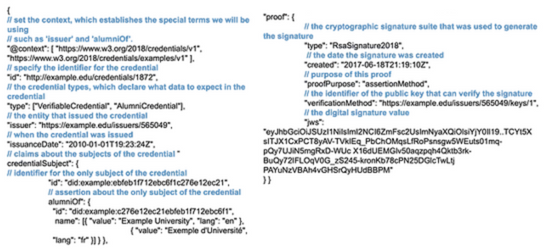
\includegraphics[width=1\textwidth]{Images/c4_3.png} 
  \caption{A simple example of verifiable credential.}
\end{figure}

\subsubsection{Verifiable Presentations}

\gls{vp}s are verifiable proofs of a person's claims that only provide selective disclosure of identity data to verifiers \cite{w3cvcdatamodel}. They are usually derived or 
generated from one or more \gls{vc}s that have metadata and crypto signatures that can be verified by the recipient. Credentials from different sources are combined through 
\gls{vp} which allow fast and privacy-preserving interactions within the \gls{ssi} framework \cite{9333857}.

\begin{figure}[h]  
  \centering
  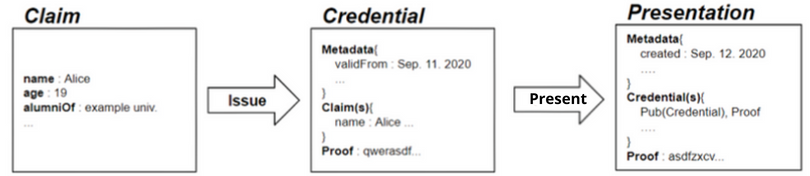
\includegraphics[width=1\textwidth]{Images/c4_4.png} 
  \caption{Core data model in W3C's VC.}
\end{figure}

\subsubsection{Zero-Knowledge Proof}

\gls{zkp}s are a type of proof that allows one to demonstrate a value without actually revealing the value itself \cite{w3cvcdatamodel}. Essentially, \gls{zkp}s provide privacy 
and support selective discloser of credential attributes in the VCs ecosystem. The \gls{zkp}s enable hidden proving with the provision holding claims of participants without 
revealing the sensitive information, they provide privacy-protecting interactions in the \gls{ssi} ecosystems. This provides the opportunity to issue zero-knowledge verifiable 
proofs of possession, to allow holders to disclose important information without revealing their secret. This conceals the information disclosed to verifiers by individuals 
utilizing \gls{zkp}s while remaining in charge of their personal data.

\subsection{Verifiable Data Registries}

Verifiable data registries form a key pillar in \gls{ssi} systems which provide a decentralized mechanism for the secure storage of identity-related data
such as \gls{did}s and \gls{vc}s. These registries guarantee the validity and reliability of the data without any need to the 
central authority \cite{w3cvcdatamodel}.

\subsubsection{Blockchain as a Distributed Verifiable Data Registry} 

Blockchains provide distributed verifiable data registries as a critical feature for \gls{ssi} infrastructures. Being a distributed ledger technology, blockchains ensures 
immutability and decentralization, which makes them a perfect choice, for recording and validating transactions in a trustless environment \cite{9869618}.

In the case of blockchain-based \gls{ssi} frameworks, the transactions containing the assertions of the identity and the verifications of these assertions are recorded in blocks 
linked chronologically. Each block is given a cryptographic hash of the previous block, thus the blockchain is made secure and the ledger is done without interruption. 
Through cryptographic signatures of stored data and events, Blockchains provide a tamper-proof encryption repository for identity data.

\subsubsection{Distributed Hash Table in SSI}

As in blockchain, \gls{dht}s ensures a decentralized way of storage and retrieval of data within the scope of \gls{ssi} frameworks. \gls{dht}s are the decentralized 
data store components and are known for their rapid lookup capabilities based on the key-value pair \cite{9869618}. Technology platforms such as the \gls{ipfs} 
utilize \gls{dht}s to make the storage and retrieval of archival data more efficient, increasing the overall performance and improving the decentralization of content delivery.

\gls{ipfs} utilizes the \gls{dht} technology, distributing data across multiple nodes of a decentralized peer-to-peer network. Such an approach not only increases data resilience and 
availability, but also minimizes the dependence on a centralized server for data retrieval. In addition, the \gls{dht} structure used in systems like \gls{ipfs} facilitates content 
addressing, which makes it possible for users to retrieve the data using the unique hash addresses while not having to depend on any centralized storage infrastructures.

\section{Architecture of Decentralized Identity} 

The Decentralized Identity architectural framework consists of four layers that correspond to different building blocks, each of them being a critical part in implementation
and operation of the system. Such layers are built to offer trust and smoothen interactions among parties existing in the decentralized identity ecosystem. The 
implementation of this infrastructure is based on the works of the pioneers in the field, including papers from the Trust over \gls{ip} Foundation \cite{DIDarchitecture}.

\subsection{The Four Layers} 

\begin{figure}[h]  
  \centering
  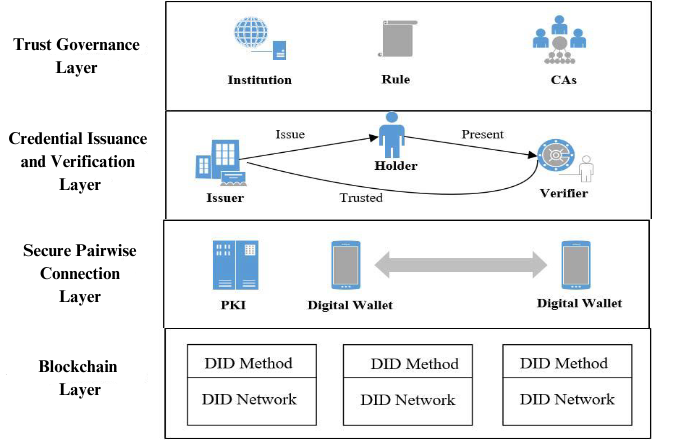
\includegraphics[width=0.8\textwidth]{Images/c4_5.png} 
  \caption{SSI architecture.}
\end{figure}

\begin{enumerate}
  \item \textbf{Blockchain Layer (Layer 1)}:
  \begin{itemize}
    \item It works as a base layer, making a retrievable data registry and storage for \gls{did}s and the associated \gls{ddo}s \cite{DIDarchitecture}.
    \item Deals with the definition, storage and management of \gls{vc}s and their definitions, schemas and descriptions respectively.
    \item It facilitates credential revocation by maintaining the Revocation Registry record when a credential issuer revokes a credential.
    \item Incorporates proof of consent mechanisms for the exchange of data among entities securely.
  \end{itemize}
  
  \item \textbf{Secure Pairwise Connections Layer (Layer 2)}:
  \begin{itemize}
    \item Enables secure communication between agents and digital wallets through share pairwise links.
    \item Is in charge of the creation and maintenance of secure links between two parties, which are the agents.
    \item It makes communication of personal messages safely through encrypting and decrypting.
    \item Its job is to deal with the digital wallet information, guaranteeing the secure storage and management of credentials.
  \end{itemize}
  
  \item \textbf{Credential Issuance and Verification Layer (Layer 3)}:
  \begin{itemize}
    \item Enables the issuer to issue \gls{vc}s to holders in order to form the trust triangle.
    \item Enables the holders to have their digital wallets and accommodate the credentials from multiple issuers.
    \item Provides ability to combine different claims from several \gls{vc}s into one complex compound proof for attestation.
    \item Enables verifiers to verify the holder's proof using the \gls{vc}s and disregarding the issuer.
  \end{itemize}
  
  \item \textbf{Trust Governance Layer (Layer 4)}:
  \begin{itemize}
    \item Establishes governance structures, policies, and contracts to build up trust among parties participating in the ecosystem.
    \item Specify a set of rules in which entities can stay within the guidelines of the decentralized identity system.
    \item Uses Trust Anchors, Auditors, or known governance organizations which are responsible for issuer and verifier’s integrity.
  \end{itemize}
\end{enumerate}

The security measures are implemented across the layers 1 and 2, using cryptography primarily \cite{DIDarchitecture}. This helps improve security to a great extent. These tasks range from the 
generation of public and private keys through the associated cryptographic operations during the interval of credential lifecycle (issuing, generating, verifying, and 
revocation), and to the encryption and decryption of messages that are exchanged between wallets and agents.

\section{The SSI Trust Triangle}

In the realm of decentralized identity management, the \gls{ssi} architecture operates on the basis of a trust triangle involving three primary actors: 
Holder, Issuer and Verifier. Clearly, the role and interactions of these components are the determining factor in understanding the dynamics of decentralized identity systems.

\subsection{Key Actors of SSI}

\begin{itemize}
  \item \textbf{Holder}: The Holder is the identity of the individual user within the decentralized identity ecosystem. Equipped with a digital wallet application, the 
  Holder generates their \gls{did}s. The \gls{did} acts as a unique identifier for the user and belongs to a digital wallet in which \gls{vc}s are stored. \gls{vc}s are 
  cryptographic attestations, which are issued by trusted parties, the Issuers \cite{dockio}.
  \item \textbf{Issuer}: Issuers are the organizations or entities that are responsible for verifying the identities of users and issuing \gls{vc}s. These 
  credentials are signed with the Issuer's private key and therefore establish the authenticity and integrity of the information contained within. After the verification, 
  the VC is linked with the Holder's \gls{did} and it is stored in their digital wallet.
  \item \textbf{Verifier}: Verifiers are entities that use the provided \gls{vc}s to verify the users' identities. Upon the presentation of the Holder's 
  credentials by the Holder, the Verifier runs the public \gls{did} on the blockchain to confirm the credibility of the issuer. The verification of the cryptographic signatures 
  embedded within the credentials by the Verifier ensures that the presented information was not tampered with and originates from a trusted source.
\end{itemize}
 
\begin{figure}[h]  
  \centering
  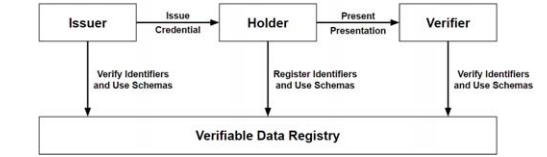
\includegraphics[width=1\textwidth]{Images/c4_6.png} 
  \caption{Basic concept of W3C's VC.}
\end{figure}

\subsection{Workflow of Verifiable Exchange}

\begin{enumerate}
  \item \textbf{Creation of Decentralized Identity}:
  Users start the whole procedure by generating a \gls{did} for each piece of data that they want to share. This \gls{did} functions as the user's identification post within the 
  decentralized network in a cryptographic manner \cite{ciscofpie}.
  \item \textbf{Issuance and Validation of Verifiable Credentials}:
  On request, an Issuer validates the Holder’s \gls{did} usually by referring to an immutable public ledger. After validation, the issuer creates and signs the \gls{vc} 
  containing the relevant information. This credential is paired with Holder's \gls{did} and stored in their digital wallet.
  \item \textbf{Presentation of Verifiable Credentials}:
  The Holder uses the stored \gls{vc}s in their digital wallet to establish a specific claim. Through signing the provided credential, the Holder builds a 
  \gls{vp} of their claimed identity.
  \item \textbf{Verification by the Verifier}:
  After receiving the presentation, the Verifier performs a set of verifications to ensure its authenticity is intact. This process entails checking the cryptographic 
  signatures appearing in the credentials and authenticating the nearest public \gls{did}s on the blockchain. The Verifier confirms the authenticity of the delivered information 
  and thus guarantees the credibility of the reported identity \cite{9869618}.
\end{enumerate}